\section{Brukergrensesnitt \texttt{(View)}} \label{sec:brukergrensesnitt}

Dette deltkapittelet er litt overlappende med kapittelet "Swing-komponenter". Les gjerne mer om det her \ref{sec:swing} \pageref{sec:swing}.

\subsection{Oppstart av brukergrensesnittet}
I \texttt{MainController.java} instansieres først to Arkfaner, \texttt{ArkfaneMegler.java} og \texttt{ArkfaneAnnonse.java}.
Disse sendes så med som parametere inn i strukturen til brukergrensesnittet, først til \texttt{StartGUI.java}, og så videre til \texttt{MainPanel.java} som oppretter \texttt{JTabbedPane} og legger inn de to arkfanene der.
Grunnen til at arkfanene ble opprettet allerede i \texttt{MainController.java} er fordi vi sender med det respektive arkfane under instansiering av \texttt{Kontrollerne}. 
Siden de to arkfanene har så lik funksjonalitet, deler de på \texttt{Kontrollerne} som de har felles.

Fra \texttt{MainController.java} opprettes det to versjoner av \texttt{ControllerTabell.java}. Til den ene sendes vinduet \texttt{meglerVindu} som er instans av \texttt{ArkfaneMegler.java} og til den andre kontrollerinstansen sendes \texttt{annonseVindu} som er instans av \texttt{ArkfaneAnnonse.java}.
Se illustrasjonen nedenfor.
\begin{figure}[ht]
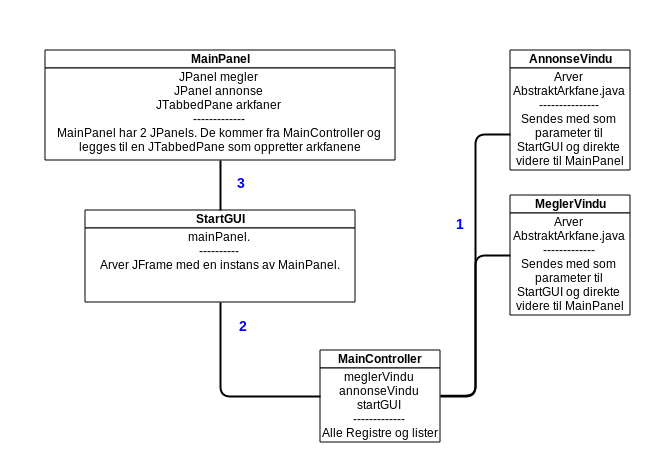
\includegraphics[width=\textwidth,height=\textheight,keepaspectratio]{./img/produktdokumentasjon/bilder/Controller_og_GUI-opprettelse2.png}
\caption{Illustrasjon over hvordan \texttt{MainController} starter opp programmet}
\end{figure}


\subsection{Bruk av arv i brukergrensesnittet}
Brukergrensesnitt er utrolig tidkrevende å jobbe med, og veldig mye av det man gjør er å skrive samme kode for hvert enkelt vindu.
For å unngå dette mest mulig, samt å få alle vinduer og paneler til å ha mest mulig den samme følelsen har vi noen abstrakte klasser som vi arver på tvers av alle klassene som har med brukergrensesnitt å gjøre.


\subsubsection*{\texttt{AbstractPanel.java}}
Dette panelet arver \texttt{JPanel} og er superklassen til alle andre hovedvinduer og paneler i programmet.
Denne klassen har to \texttt{konstruktører}. Den ene tar inn to heltall som representerer bredde og høyde på det panelet som arver klassen, samt en \texttt{String borderTitle} som blir tittel på kantlinjen som \texttt{konstruktøren} oppretter.
Den andre \texttt{konstruktøren} er omtrent lik, men tar ikke inn en \texttt{String} for kantlinje, så her kan man velge mellom to \texttt{konstruktører}, med eller uten kantlinje.
Dette panelet er også satt med en bakgrunnsfarge slik at alle paneler og vinduer som arver denne vil arve denne.

\texttt{CustomSubPanel.java} arver også \texttt{AbstractPanel.java}. Denne klassen brukes i hovedsak for paneler inne i et hovedpanel. Da dette panelet skal brukes gjentatte ganger i mange forskjellige sammenhenger er det hele 6 \texttt{konstruktører} her. 
I noen opprettes det en predefinert \texttt{Layout}, i andre ikke. Noen tar inn størrelse (bredde og høyde), andre ikke. På denne måten har vi fått en veldig slagkraftig klasse som har spart oss for mye arbeid og forenklet konstruksjonen av brukergrensesnitter veldig.


\subsubsection*{\texttt{AbstractRegistreringsVindu.java} og \texttt{AbstractRegistreringsPanel.java}}
\texttt{AbstractRegistreringsVindu.java} er superklassen for \texttt{AbstractRegistreringsPanel.java}. Denne klassen arver \texttt{JFrame} og er setter de mest generelle parameterne som et hvert vindu skal ha. Størrelse, navn på vinduet, samt standard lukkefunksjonalitet osv.
\texttt{AbstractRegistreringsPanel.java} er superklassen til alle registreringsvinduene. Denne klassen har en \texttt{BorderLayout} og tar inn parametere som bredde, høyde og tittel for vinduet som opprettes. Ut over dette gjør ikke denne klassen mye. Alle klasser som arver denne vil velge hvilke paneler fra denne klassens \texttt{BorderLayout} de ønsker å ta i bruk.


\subsection{Oppbyggningen av arkfanene}
Begge arkfanene er bygget over samme lest. De arver \texttt{AbstraktArkfane.java}. Denne klassen tar inn en \texttt{String} som avgjør hvilke \texttt{topPanel} som skal følge med arkfanen.
\texttt{AbstraktArkfane.java} består i korte trekk av en \texttt{BorderLayout} med fire paneler; \texttt{toppanel, venstrepanel, senterpanel} og \texttt{bunnpanel}.
Hvert av panelene er satt opp med en \texttt{get-metode} som brukes hyppig av \texttt{kontrollerne} i kommunikasjonen med komponentene der.

Alle \texttt{kontrollerne} er "klar" over sitt vindu, og nedenfor er et eksempel på hvordan \texttt{ControllerTabell.java} kommuniserer med vinduet.

\begin{lstlisting}[caption=Kodeeksempel på hvordan \texttt{ControllerTabell.java} kommuniserer med brukergrensesnittet]
        /**
         * Lytter på museklikk i Output-vinduet.
         */
        vindu.getSenterpanel().getEditorPane().addMouseListener(new MouseAdapter() {

            @Override
            public void mouseClicked(MouseEvent e) {
                if (e.getButton() == MouseEvent.BUTTON1) {
                    if (modellIBruk instanceof TabellModellAnnonse) {
                        Annonse valgtObjekt = returnerAnnonseObjekt();
                        if (vindu instanceof ArkfaneMegler) {
                            new ControllerBildeViser(valgtObjekt.getBolig(), true);
                        } else {
                            new ControllerBildeViser(valgtObjekt.getBolig(), false);
                        }
                    }
                }
            }

        });
\end{lstlisting}

I figuren ovenfor kan man både få tak i \texttt{vindu} sine paneler, men også teste om \texttt{vindu} er av type \texttt{ArkfaneMegler} eller ikke. Tidligere i prosjektet brukte vi \texttt{konstanter} som ble sendt med som parametere for å identifisere hvilke vindu man var i, og hvilken objekttype man behandlet til en hver tid.


\subsubsection*{\texttt{TopPanelMegler.java, TopPanelAnnonse.java, VenstrePanel.java, SenterPanel.java} og \texttt{BunnPanel.java}}
De tre nevnte panelene utgjør innholdet i hver av arkfanene. 
Da all funksjonalitet finnes i de respektive \texttt{kontrollerne} er hver av disse klassene ganske små. De består i grunn bare av en \texttt{Layout} samt den/de komponentene som vises, inkludert subpaneler samt \texttt{get-metoder} en trenger for å kunne hente informasjon derfra.
Det er brukt forskjellige \texttt{Layout-managere}, alt etter hvilken som er mest hensiktsmessig i den gitte situasjon.
I \texttt{VenstraPanel.java} og \texttt{SenterPanel.java} har man bare én komponent hver som dominerer hele panelet, men \texttt{kontrollerne} bak disse er desto større.
\texttt{JTable} i \texttt{VenstrePanel.java} har utrolig mye funksjonalitet og er hjerte i hele programmet.
\texttt{JEditorPane} i \texttt{SenterPanel.java} er en ren \texttt{output-pane} som skriver ut html-visning av objektene i tabellen. 


\subsection{Registreringsvinduene}
Registreringsvinduene er bygget over samme lest, og arver \texttt{AbstractRegistreringsPanel}. De er likevel ganske forskjellige. De bruker et utall forskjellige \texttt{Layout-managere}, og ofte en blanding mellom flere. 
\texttt{GridBagLayout} er likevel den mest allsidige og foretrukne \texttt{Layout-manageren} vi har brukt. 

Så og si alle komponentene vi har brukt er \texttt{Custom...}. Det vil si egendefinerte komponenter vi har laget, og som arver den opprinnelige \texttt{Swing}-komponenten. 
Det beste eksempelet her er \texttt{CustomJTextField.java} som blant annet tar inn et \texttt{String pattern} som er en \texttt{RegEx}-konstant, slik at komponenten har innebygget \texttt{RegEx}-funksjonalitet.

Alle registreringsvinduene har i sine \texttt{kontrollere} egne \texttt{konstruktører} ment for nye objektet og for endring av objektene. Det vil si at når en endrer et objekt så fylles komponentene ut med relevant informasjon fra det innkomne objektet.

Når en velger ny \texttt{Bolig} eller har valgt et valg som gjelder bare for én type objekter så vil de valgene som ikke gjelder for det valget bli deaktivert og ikke mulig å legge inn informasjon på. Dette er selvfølgelig funksjonalitet som ligger i \texttt{kontrollerne} og vil bli nevnt i \ref{sec:regkontrollere} på side \pageref{sec:regkontrollere}.

Vi har gjort et eksperiment med \texttt{PersonRegVindu.java}. 
Dette er et felles registreringsvindu for både \texttt{Leietakere} og for \texttt{Utleiere}. Vinduet har to \texttt{kontrollere} som kaller på vinduet ved behov.
Dette betyr at en del komponenter vil være overflødige i noen tilfeller, og nødvendige i andre tilfeller. Dette vil bli nevnt mer i \ref{sec:regkontrollere} på side \pageref{sec:regkontrollere}.

